We begin by studying a ``toy model'' of floating-point numbers.

\begin{defn}
  Let $\beta\in\NN$ be greater than 1, $t\in\NN$. The
  \define{Idealized Floating Point} in base $\beta$ with precision $t$
  consists of the set
  \begin{equation}
    \FF_{\beta,t} = \{\, (s,m,e)\mid s=\pm1, 0\leq m<\beta^{t},e\in\ZZ\,\}
  \end{equation}
  where $m$ is the \define{Mantissa}, $s$ is the \define{Sign}, and $e$ is the
  \define{Exponent}. We interpret $(s,m,e)$ as the rational number
  \begin{equation}
    \fl^{-1}_{\beta,t}(s,m,e) = s(m/\beta^{t})\beta^{e}\in\QQ
  \end{equation}
  and $\fl_{\beta,t}\colon\RR\to\FF_{\beta,t}$ encodes a real number as an
  idealized floating point number.
\end{defn}

\begin{rmk}[Uniqueness of float]
We adopt the convention that $\beta^{t-1}\leq m<\beta^{t}$ \emph{or} $m=0=e$, otherwise there are
multiple encodings of the same number --- for example $(0,t-1,1)$ and
$(0,t,0)$ encode the same number. We want \emph{exactly one} choice for
encoding a real number as a floating point number, so we can describe it
as a function.
\end{rmk}

\begin{rmk}[Standard values for $\beta$, $t$]
  The \ieee-754 standard specifies that $\beta=2$ or $\beta=10$. Further,
  for $t$, we have the following table of possible values:
\begin{table}[h!]
  \centering
  \begin{tabular}{ |c|c|c| }
    \hline
 Name              & $\beta=2$ & $\beta=10$ \\ \hline
 Single Precision  & 24  & 7 \\  
 Double Precision  & 53  & 16\\
 Quad Presision    & 113 & 34\\
 Octuple Precision & 237 & 71(?)\\
 \hline
\end{tabular}
\caption{Table of precision in various bases; note: there is no
  \ieee\ standard for $\beta=10$ Octuple precision.}
\end{table}
\end{rmk}

\begin{rmk}[On ``Idealization'']
  The idealization we have implicit in this model is that the exponent
  may be an arbitrary integer. In the real world, floating point numbers
  have the exponent be an integer between $e_{\text{min}}\leq e\leq e_{\text{max}}$.
  The only difference is overflow is not a concern with idealized
  floating-point arithmetic.
\end{rmk}

\begin{rmk}[Abuse of notation]
We will often write floating point numbers ``as if'' they were a subset
of $\QQ$. So instead of writing $(1,1,1)$ we'll just write $-\beta$.
\end{rmk}

\begin{convention}
  We will use the variables $u$, $v$, $w$ for floating-point numbers. 
  We will let $x$, $y$, $z$ range over ``actual numbers'' (either $\RR$
  or $\QQ$).
\end{convention}

\begin{defn}
Let $\FF_{\beta,t}$ be idealized floating point numbers with base
$\beta$ and precision $t$. The \define{Encoding Map} is a surjective
function
\begin{equation}
  \fl_{\beta,t}\colon\RR\onto\FF_{\beta,t}
\end{equation}
such that it is ``exact'' on encodable rational numbers $\pm(m/\beta^{t})\beta^{e}\in\QQ$
is mapped to $(s,m,e)$; further, its ``decoding map'' is
\begin{equation}
  \fl_{\beta,t}^{-1}(s,m,e) = (-1)^{s}(m/\beta^{t})\beta^{e}.
\end{equation}
\end{defn}

\begin{thm}
  We see that $\fl\circ\fl^{-1}=\id$.
\end{thm}

\subsection{Rounding Schemes}

\begin{rmk}[Rounding schemes]
  Implicit underlying $\fl_{\beta,t}$ is a choice of rounding. If
  $x = (-1)^{s}(m/\beta^{t})\beta^{e}$ for some $s\in\{0,1\}$,
  $\beta/2\leq m<\beta$, and $e\in\ZZ$, and if $|\delta x| < \beta^{e-t}$,
  then we need to determine how to encode $x + \delta x$.

  We will write $R(x+\delta x)$ for some rounding scheme $R(-)$ encoding
  a real number $x+\delta x$ to its nearest floating-point number.
\end{rmk}
\begin{notation}
  We may abuse notation, writing $R(s,m+k,e)$ for rounding the rational
  number $(-1)^{s}((m+k)/\beta^{t})\beta^{e}$ to its nearest
  floating-point number. If this seems silly, consider the case when
  $m=\beta^{t}-1$ and $k=2$: $(s,m+k,e)$ is not a valid floating-point
  number. But $R(s,m+k,e)$ would produce a correct floating-point
  number, rounded as needed.
\end{notation}

\begin{defn}
  \define{Truncation} (or ``rounding towards zero'') is a rounding
  scheme which literally throws away
  $\delta x$, so
  $\RZ(x+\delta x)=\fl_{\beta,t}(x)$ for $0\leq\delta x<\beta^{e-t-1}$.
\end{defn}


\begin{defn}
  The default for \ieee-754 arithmetic is
  \define{Round Half-to-Even},
  denoted $\RN_{\text{even}}(x)$:\marginpar{Round half-to-even, default \ieee-754 scheme}
  if
  \begin{equation}
    \begin{split}
      \delta x &= (-1)^{s'}(m'/\beta^{t})\beta^{e'}\\
      &= (-1)^{s'}(\delta m/\beta^{t})\beta^{e}
    \end{split}
  \end{equation}
  as a rational number, then we have several case:
  \begin{itemize}
    \item Case 1: if $\delta m<1/2$, then $\RN_{\text{even}}(x+\delta x)=\RN_{\text{even}}(x)$
    \item Case 2: if $\delta m\geq1/2$
      \begin{itemize}
        \item Subcase 1: if $m$ is even, then $\RN_{\text{even}}(x+\delta x)=\RN_{\text{even}}(x)$
        \item Subcase 2: if $m$ is odd, then $\RN_{\text{even}}(x+\delta x)=(s,m+(-1)^{s'},e)$
      \end{itemize}
  \end{itemize}
  Observe for $\beta=2$, this simplifies to examining the last bit in
  the mantissa of $x$ to see if it's even (i.e., 0) or odd (i.e., 1),
  and $\delta x$ has $e'=e-t$ (which encodes $\delta m\geq1/2$) or
  $e'<e-t$ (encoding $\delta m<1/2$).
\end{defn}

\begin{rmk}
  For $\beta=2$, we can treat $m+\delta m$ as a $t+1$ bit number
  (truncating $\delta m$ to the leading bit). If the last two bits of
  $m+\delta m$ (as a truncated $t+1$ bit number) are
  $(11)_{2}$ in base-2, then $\RN_{\text{even}}(s,m+\delta m,e)=(s,m+1,e)$.
  Otherwise $\RN_{\text{even}}(s,m+\delta m,e)=(s,m,e)$. Since this
  scheme requires only one extra bit, it is easier to implement in
  hardware compared to other schemes.
\end{rmk}
\begin{defn}
  The familiar rule for rounding taught to elementary school students is
  called \define{Round to Nearest, Ties Away From Zero}, denoted $\RN_{\text{away}}(x)$. If the number falls
  midway, it is rounded to the nearest value above (for positive
  numbers) or below (for negative numbers). This would have
  $\RN_{\text{away}}(x+\delta x)=(s,m+\sgn(x+\delta x), e)$ provided $\delta m\geq1/2$;
  and $\RN_{\text{away}}(x+\delta x)=\fl_{\beta,t}(x)$ when $\delta m<1/2$.
  This matches intuition when working with $\beta=10$.
\end{defn}

\begin{notation}
  We write $\RN(x)$ for either $\RN_{\text{even}}(x)$ or $\RN_{\text{away}}(x)$,
  when it doesn't matter which one we use.
\end{notation}

\begin{thm}
  For any $x\in\RR$, we have $\RN(-x)=-\RN(x)$.
\end{thm}

\begin{notation}
In the literature, at least the \emph{Handbook of Floating-Point Arithmetic}~\cite{10.5555/3235984},
rounding is written as $\circ(x)$ whereas we have chosen a more explicit
convention using $\fl(x)$. It is common to write $\circ(x+y)$ when what
is meant is $\fl(\fl^{-1}(x)+\fl^{-1}(y))$, i.e., produce the
floating-point number corresponding to the sum of $x$ and $y$ when
treated as real numbers \emph{in some rounding scheme}.
\end{notation}

\begin{convention}
  We will follow \ieee-754 convention throughout this book, and
  typically work with $\beta=2$ and $\RN_{\text{even}}(-)$ rounding scheme.
  Hence $\fl_{2,t}\colon\RR\to\FF_{2,t}$ generically maps $x\in\RR$ to
  $\RN_{\text{even}}(x)$.
\end{convention}

\begin{thm}
Encoding real numbers as floating-point numbers is not bijective, but it
is surjective for any rounding-scheme.
\end{thm}
\begin{proof}
To prove $\fl_{\beta,t}$ is surjective, we see that for any $(s,m,e)\in\FF_{\beta,t}$,
there is a real number which maps to it, namely:
\begin{equation}
  \fl((-1)^{s}(m/\beta^{t})\beta^{e}) = (s,m,e)
\end{equation}
for each $s\in\{0,1\}$, $m\in\{\beta/2,\dots,\beta-1\}$, and $e\in\ZZ$.

Now, to prove it's not bijective, we just need to prove it's not
injective. Take $x = (-1)^{s}(m/\beta^{t})\beta^{e}\in\QQ$. Then for
any real number $\delta x$ with its mantissa $\delta m$ satisfying
$0\leq \delta m<\beta^{t-1}/2$, we see
\begin{equation}
  \fl_{\beta,t}(x + \delta x) = \fl_{\beta,t}(x).
\end{equation}
Hence $\fl_{\beta,t}$ is surjective but not injective.
\end{proof}

\begin{ex}
  Let's look at a few constants, just to see what they look like. We find
  \begin{equation}
    \fl_{\beta,t}(1) = (0, \beta^{t-1}, 1-t)
  \end{equation}
  and
  \begin{equation}
    \fl_{\beta,t}(2) = \begin{cases}
      (0, 1, 1) & \mbox{if $\beta=2$}\\
      (0, 2\beta^{t-1}, 1-t)  & \mbox{if $\beta>2$}.
    \end{cases}
  \end{equation}
  Hence
  \begin{equation}
    \fl_{\beta,t}(1/2) = \begin{cases}
      (0, 1, -1) & \mbox{if $\beta=2$}\\
      (0, \beta^{t}/2, 1-t)  & \mbox{if $\beta>2$}.
    \end{cases}
  \end{equation}
  Observe for $\beta=3$ (or any odd integer $\beta$), it is impossible
  to encode $1/2$ exactly.
\end{ex}

\begin{ex}\label{ex:idealized-floating-point:eleven-point-five}
  In $\beta=10$, with $t=1$, what do the idealized floating point numbers
  look like? We'd have
  \begin{equation}
    S = \{\,1,2,3,4,5,6,7,8,9\,\}
  \end{equation}
  and then we can construct the numbers:
  \begin{equation}
    \FF_{10,1} = \fl_{10,1}\left(\bigcup_{n\in\ZZ}-10^{n}S\right)\cup
    \fl_{10,1}\left(\bigcup_{n\in\ZZ}10^{n}S\right).
  \end{equation}
  How do we encode, say, $10.5$ in this system? We have only 1 digit in
  the mantissa, so we would have to round to the nearest
  number\footnote{There are other rounding schemes possible, e.g.,
  ``always round down'', ``always round up'', rounding towards infinity,
  etc.}. For this particular system, we have the distribution of numbers
  schematically depicted in figure~\ref{fig:img-0}. We see that
  $\fl_{10,1}(10.5)=(0,1,1)$ --- i.e., it's encoded as 10.

  \begin{figure}[t]\label{fig:img-0}
    \centering
    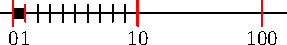
\includegraphics{img/img-0.mps}
    \caption{Distribution of positive floating point numbers in base
      $\beta=10$ with $t=1$ digits of precision.}
  \end{figure}
\end{ex}

\begin{thm}
Ideal floating point numbers do not contain the integers.
\end{thm}
\begin{proof}
It suffices to show that $\ZZ\not\subset\fl_{\beta,t}^{-1}(\FF_{\beta,t})$.
For example $\beta^{t}+1$ is not a possible floating-point number.
\end{proof}
\begin{cor}\label{cor:ideal-floats:ints-representable-by-floats}
Any integer $k\in\ZZ$ such that $|k|<\beta^{t}$ may be encoded in
$\FF_{\beta,t}$ exactly.
\end{cor}
\begin{proof}
  Without loss of generality, let's work with $k>0$ since $k=0$
  corresponds to $(0,0,0)$ and $k<0$ amounts to just changing the sign.

  \textsc{Case 1:} $\beta^{t-1}\leq k<\beta^{t}$. Then $(0,k,0)$ encodes
  $k$ exactly.

  \textsc{Case 2:} $0<k<\beta^{t-1}$. Suppose that $s$ is the smallest
  positive integer such that $\beta^{s-1}\leq k<\beta^{s}$. Then we
  claim $(0, \beta^{t-s}k, s-t)$ encodes $k$ exactly:
  $\beta^{s-1}\beta^{t-s}=\beta^{t-1}\leq \beta^{t-s}k < \beta^{s}\beta^{t-s}$
  is a valid mantissa, and $s-t$ is a valid exponent.
\end{proof}

\begin{puzzle}
Can we measure ``how good'' (or ``how bad'') $\fl_{\beta,t}(x)$
approximates $x$?
\end{puzzle}

\begin{defn}\label{defn:absolute-error}\label{defn:relative-error}
  Let $\widehat{x}\in\RR$ be an approximation to $x\in\RR$. Its
  \define{Absolute Error} is
  \begin{equation}
    \varepsilon_{\text{abs}} = |\widehat{x} - x|.
  \end{equation}
  If $x\neq0$, then the \define{Relative Error} of the approximation is
  \begin{equation}
    \varepsilon_{\text{rel}} = \left|\frac{\widehat{x}-x}{x}\right|.
  \end{equation}
\end{defn}

\begin{xca}
What is the relative and absolute error of $\pi$ as an approximation to $\sqrt{10}$?
\end{xca}
\begin{xca}
What is the relative and absolute error of $2^{10}$ and $3^{19/3}$ as an
approximation to $10^{3}$?
\end{xca}

\begin{defn}\label{defn:round-off-error}
Let $\FF_{\beta,t}$ be idealized floating point numbers with base
$\beta$ and precision $t$, let $x\in\RR$ be some real number. The
\define{Absolute Round-Off Error} encoding $x$ as a floating point number is
\begin{equation}
\roundError_{\beta,t;\text{abs}}(x) = |x - \fl_{\beta,t}^{-1}(\fl_{\beta,t}(x))|.
\end{equation}
The \define{Relative Round-Off Error} encoding $x$ is
\begin{equation}
\roundError_{\beta,t;\text{rel}}(x) = \left|\frac{x - \fl_{\beta,t}^{-1}(\fl_{\beta,t}(x))}{x}\right|,
\end{equation}
provided $x\neq0$.
\end{defn}

\begin{ex}
  Continuing
  example~\ref{ex:idealized-floating-point:eleven-point-five},
  the round-off error for $11.5$ in $\FF_{10,1}$ is
  \begin{equation}
    \roundError_{10,1;\text{abs}}(11.5) = |11.5 - 10| = 1.5
  \end{equation}
  and the relative round-off error is
  \begin{equation}
    \roundError_{10,1;\text{rel}}(11.5) = \frac{|11.5 - 10|}{11.5} = 2/23\approx 0.1304348
  \end{equation}
\end{ex}

\begin{puzzle}
Is there an upper bound to the relative round-off error? If so, what is it?
\end{puzzle}

\subsection{Bounds on Round-Off Error}


\begin{lemma}
In $\FF_{10,1}$, the relative round-off error is maximum for $x\in\RR$
such that it lies half-way between two numbers $x_{0}<x<x_{1}$ for
$x_{0},x_{1}\in\fl_{10,1}^{-1}(\FF_{10,1})$.
\end{lemma}
\begin{proof}
Regardless of rounding, we see that $\fl_{10,1}(x)$ will be either
$\fl_{10,1}(x_{0})$ or $\fl_{10,1}(x_{1})$. But $x_{1}-x_{0}=10^{e}$
where $\fl_{10,1}*x(=(s,m,e)$.
The relative round-off error would then be
\begin{equation}
  \roundError_{10,1;\text{rel}}(x) = \frac{10^{e}/2}{|x|} = \frac{10}{2}.
\end{equation}
The reason for $10^{e}/2$ is because $x$ is \emph{half-way} between
$x_{0}$ and $x_{1}$.
\end{proof}

\begin{lemma}\label{lemma:idealized:truncation-round-off-error}
In $\FF_{\beta,t}$, the round-off error for truncation rounding is
bounded by $\beta^{1-t}$
\end{lemma}
\begin{proof}
  In base $\beta$, write $x=d_{0}.d_{1}d_{2}\dots d_{t-1}d_{t}\dots\times\beta^{e}$ for
  its expansion in that base. We then have
  \begin{equation}
    \begin{split}
      \roundError_{\beta,t;\text{rel}}(x) &=
      \left|\frac{(d_{t}.d_{t+1}\dots)\times\beta^{e-t}}{d_{0}.d_{1}\dots d_{t-1}\times\beta^{e}}\right| \\
      &=
      \frac{(d_{t}.d_{t+1}\dots)}{d_{0}.d_{1}\dots d_{t-1}}\times\beta^{-t} 
    \end{split}
  \end{equation}
  The denominator is greater than 1, the numerator is bounded by
  $\beta-1$, so we have
  \begin{equation}
    \roundError_{\beta,t;\text{rel}}(x) \leq\beta^{1-t}
  \end{equation}
  as claimed.
\end{proof}  
\begin{proof}[Alternate Proof]
Let $x = (-1)^{s}((m + \delta m)/\beta^{t})\beta^{e}\in\QQ$ where
$0 < \delta m < \beta^{t-1}$, $\beta^{t-1}\leq m<\beta^{t}$, $s\in\{0,1\}$,
and $e\in\ZZ$. Then $\fl_{\beta,t}(x) = (s,m,e)$ and the round-off error
is
\begin{equation}
  \roundError_{\beta,t;\text{rel}}(x)
  = \frac{(\delta m/\beta^{t})\times\beta^{e}}{((m+\delta m)/\beta^{t})\times\beta^{e}}
  = \frac{\delta m}{m+\delta m}
\end{equation}
where the denominator has $\beta^{t-1}\leq m$ give us the bound
\begin{equation}
  \roundError_{\beta,t;\text{rel}}(x)\leq\frac{\delta
    m}{\beta^{t-1}+\delta m} = \frac{\beta^{1-t}}{1 + (\delta m)^{-1}} < \beta^{1-t}
\end{equation}
precisely as asserted.
\end{proof}

\begin{lemma}\label{lemma:idealized:rn-round-off-error}
In $\FF_{\beta,t}$, the round-off error for round-to-nearest rounding is
bounded by $\beta^{1-t}/2$
\end{lemma}

\begin{proof}
Let $x=((m+\delta m)/\beta^{t})\beta^{e}$ for some integer $\beta^{t-1}\leq m<\beta^{t}$
and real $0<\delta m<\beta^{t-1}$, and $e\in\ZZ$. We are assuming $x>0$
for simplicity (the proof for $x<0$ is the same). 

Observe that $(x - \fl^{-1}_{\beta,t}(\fl_{\beta,t}(x)))\beta^{t-e}\leq \frac{1}{2}\beta$.
That is to say, in base $\beta$, the expansion $x = (d_{0}.d_{1}\dots d_{t-1}d_{t}d_{t+1}\dots)\beta^{e}$
has $(\fl^{-1}\circ\fl_{\beta,t})(x) - x\leq (\beta -d_{t})\beta^{-t-1}\beta^{e}$. Hence
\begin{equation}
  \roundError_{\beta,t;\text{abs}}(x)\leq
  \frac{(\beta/2)\beta^{-t-1}\beta^{e}}{((m+\delta m)/\beta^{t})\beta^{e}}
\end{equation}
Then using the lower-bound $\beta^{t-1}< m+\delta m$ gives us
\begin{equation*}
  \roundError_{\beta,t;\text{abs}}(x) < \frac{1}{2}\beta^{1-t}.\qedhere
\end{equation*}
\end{proof}


\begin{thm}
  In $\FF_{\beta,t}$, the relative round-off error is bounded by either
  $\beta^{1-t}$ or $\beta^{1-t}/2$ depending on choice of rounding scheme.
\end{thm}

\subsection{Machine Epsilon}

\begin{defn}\label{defn:idealized:machine-epsilon}
Let $\FF_{\beta,t}$ be idealized floating point numbers. We define
\define{Machine Epsilon} to be the number
$\varepsilon_{\text{mach}}\in\FF_{\beta,t}$ such that
\begin{equation}
\varepsilon_{\text{mach}} := \frac{\min\{x\in\FF_{\beta,t}\mid x>1\}-1}{2}.
\end{equation}
\end{defn}

\begin{ddanger}
  Different texts have different definitions of machine epsilon. Some
  texts take it to be the difference between the smallest floating-point
  number greater than one and 1 (i.e., twice what we have taken as the
  definition of machine epsilon). Other texts take it to be our
  definition. Notably, the \ieee-754 standard (2008 revision, at least)
  \emph{makes no mention of machine epsilon}. What's worse is that 
  revered authorities like Higham and Demmel \emph{disagree} on which
  definition to use. Consequently, ``machine epsilon'' is a horribly
  ambiguous term.
\end{ddanger}

\begin{thm}
  We explicitly have
  \begin{equation}
    \varepsilon_{\text{mach}} = \frac{1}{2}\beta^{1-t}.
  \end{equation}
\end{thm}
\begin{proof}
  We have $\fl_{\beta,t}(1) = (0,\beta^{t-1},1-t)$, so the smallest
  floating point number greater than 1 would be $(0,\beta^{t-1}+1,1-t)$.
  The difference between these two numbers would be
  \begin{equation}
  (0,1,1-t)=\fl_{\beta,t}(\beta^{1-t}).
  \end{equation}
  Half this quantity is, by definition, machine epsilon.
\end{proof}

\begin{rmk}
Machine epsilon is unique by construction.
\end{rmk}

\subsection{Arithmetic Operations on Floating Point Numbers}

\begin{prop}
For any $x\in\RR$, the relative error of the encoding $\fl_{\beta,t}(x)$
is bounded by machine epsilon:
\begin{equation}
  \fl^{-1}(\fl_{\beta,t}(x)) = x(1 + \varepsilon)
\end{equation}
for some $|\varepsilon|<\varepsilon_{\text{mach}}$.
\end{prop}

\begin{fundamentalAxiomFloat}[{Trefethen and Bau~\cite{trefethen1997numerical}}]
For any arithmetic operator of real numbers $\cdot\in\{+,-,\times,/\}$ there
is a corresponding operator of floating point numbers $\odot\in\{\oplus,\ominus,\otimes,\oslash\}$
which satisfies the property: for all $u,v\in\FF_{\beta,t}$ there is an
$\varepsilon\in\RR$ such that $|\varepsilon|\leq\varepsilon_{\text{mach}}$ and
\begin{equation}
  \fl^{-1}(u\odot v) = (\fl^{-1}(u)\cdot\fl^{-1}(v))(1 + \varepsilon).
\end{equation}
\end{fundamentalAxiomFloat}
\begin{rmk}
  \begin{enumerate}
  \item This is a statement about \emph{relative errors}.
  \item This can be taken as a definition of floating point operations
    $u\odot v := \fl(\fl^{-1}(u)\cdot\fl^{-1}(v))$: just translate the
    operands back to real numbers, perform the operation, then translate
    the result to floating-point numbers. The error in this case would
    be, for any $\rho,\sigma\in\RR$,
    $\fl^{-1}(\fl(\rho))=\rho(1+\varepsilon_{1})$,
    $\fl^{-1}(\fl(\sigma))=\sigma(1+\varepsilon_{2})$, and $\fl^{-1}(\fl(\rho)\odot\fl(\sigma))=(\rho(1+\varepsilon_{1})\cdot\sigma(1+\varepsilon_{2}))(1+\varepsilon_{3})$
    where $|\varepsilon_{j}|<\varepsilon_{\text{mach}}$ for
    $j=1,2,3$. The error in this case is bounded by $(1 + 2\varepsilon_{\text{mach}})$,
    since we could use the bound
    $$(\rho(1+\varepsilon_{1})\cdot\sigma(1+\varepsilon_{2}))(1+\varepsilon_{3})<(\rho(1+\varepsilon_{\text{mach}})\cdot\sigma(1+\varepsilon_{\text{mach}}))(1+\varepsilon_{3})$$
    then distributivity gives $$(\rho(1+\varepsilon_{\text{mach}})\cdot\sigma(1+\varepsilon_{\text{mach}}))(1+\varepsilon_{3})=(\rho\cdot\sigma)(1+\varepsilon_{\text{mach}})(1+\varepsilon_{3})$$
    and $(1+\varepsilon_{\text{mach}})(1+\varepsilon_{3})\leq(1 + 2\varepsilon_{\text{mach}})$.
    (Some care must be taken for division, we end up with the upper
    bound being $1+3\varepsilon_{\text{mach}}$.)
  \end{enumerate}
\end{rmk}
\begin{note}
Subtracting numbers very close to each other may lead to catastrophic
loss of precision. For example, think of some floating-point numbers of
the form $\fl(x)=(0,\beta^{t-1}+m_x,e)$ and $\fl(y)=(0,\beta^{t-1}+m_{y},e)$ where $0\leq m_{y}<m_{x}<\beta$.
Then
\begin{equation}
  \fl(x)\ominus\fl(y) = (0,\beta^{t-1}(m_{y}-m_{x}),e-(t-1)).
\end{equation}
We have lost $t-1$ digits of precision.

For a concrete example, suppose $\varepsilon=2\sqrt{2}\beta^{1-t}$ so we
have $y=1+\varepsilon$ is encoded as
$\fl(y)=1+3\varepsilon_{\text{mach}}$ and $x=1$. The ``correct'' answer
to $x-y=-2\sqrt{2}\beta^{1-t}$. But floating-point loses
everything but the leading coefficient, giving us
$\fl(x)-\fl(y)=-3\varepsilon_{\text{mach}} = -3\beta^{1-t}$.
\end{note}

Why is subtraction so horrible? Let $\fl^{-1}(\fl(x)) = x(1 + \varepsilon_{x})$
and $\fl^{-1}(\fl(y)) = y(1 + \varepsilon_{y})$. Then we would have
\begin{subequations}
  \begin{align}
    \fl^{-1}(\fl(x))-\fl^{-1}(\fl(y))
    &= x(1 + \varepsilon_{x})-y(1+\varepsilon_{y})\\
    &= x-y + (x\varepsilon_{x}-y\varepsilon_{y})\\
    &= x-y + (x-y)\left(\frac{x\varepsilon_{x}-y\varepsilon_{y}}{x-y}\right)\\
    &= x-y \left(1 + \frac{x\varepsilon_{x}-y\varepsilon_{y}}{x-y}\right)
  \end{align}
\end{subequations}
The relative error of this difference would be
\begin{equation}
  \varepsilon_{0} = \frac{x\varepsilon_{x}-y\varepsilon_{y}}{x-y}
\end{equation}
which can be arbitrarily large if $x$ is arbitrarily close to $y$.
% Fundamental axiom of floating-point is from Trefethen & Bau

\begin{lemma}[Sternbenz]
  Let $x,y\in\FF_{\beta,t}$ be floating point numbers.
  If
  \begin{equation}
    \fl^{-1}(y)/2\leq \fl^{-1}(x)\leq 2\fl^{-1}(y)
  \end{equation}
  as real numbers,
  then $x\ominus y$ may be computed exactly, in the sense that
  \begin{equation}
    \fl^{-1}(x\ominus y) = \fl^{-1}(x) - \fl^{-1}(y).
  \end{equation}
\end{lemma}

\begin{proof}
  Let $x = (0, m_{x}, e_{x})$ and $y=(0,m_{y},e_{y})$ be floating-point
  numbers in $\FF_{\beta,t}$. We see that
  \begin{equation}
   \frac{1}{\beta} < \frac{m_{x}}{m_{y}} < \beta
  \end{equation}
  under the hypothesis $y/2\leq x\leq 2y$, which implies
  \begin{equation}
    \beta^{e_{x}-e_{y}-1} < \frac{x}{y} < \beta^{e_{x}-e_{y}+1}
  \end{equation}
  The assumption $y/2\leq x\leq 2y$ is the same as $1/2\leq x/y\leq 2$,
  and taken together with $\beta>1$ 
  implies $e_{x}-e_{y}\in\{-1,0,1\}$. Let $\delta_{y}=e_{y}-e_{x}$, so
  $y = ((m_{y}\beta^{\delta_{y}})/\beta^{t})\beta^{e_{x}}$. Then we want
  to show
  \begin{equation}
    x-y = \frac{m_{x} - \beta^{\delta_{y}}m_{y}}{\beta^{t}}\beta^{e_{x}}
  \end{equation}
  can be represented exactly by some floating point number.

  Assume $y\leq x$ (so $e_{x}-e_{y}\in\{0,1\}$). (If $y > x$, the same
  logic holds, but the sign differs.) We have our hypothesis
  $y/2\leq x\leq 2y$ become $y\leq x\leq 2y$. If $e_{x}=e_{y}$, then the
  subtraction $m_{x}-m_{y}$ may be done exactly, and the result is
  trivial.

  The nontrivial case is when $e_{x}-e_{y}=1$. The claim is that
  $\beta m_{x}-m_{y}$ is represented by a valid mantissa. We observe
  that the mantissa $m_{x}$ satisfies the inequality
  \begin{subequations}
  \begin{equation}
    m_{y} \leq \beta m_{x} \leq 2m_{y}
  \end{equation}
  hence
  \begin{equation}\label{eq:sternbez-lemma:bounds-on-x-mantissa}
    \beta^{t}-1\leq \beta m_{x}\leq 2\beta^{t}-2.
  \end{equation}
  \end{subequations}
  But we see $1\leq \beta m_{x}-m_{y}\leq m_{y} < \beta^{t}$, so
  by corollary~\ref{cor:ideal-floats:ints-representable-by-floats}
  we can encode $\beta m_{x}-m_{y}$ as an idealized floating-point number.
\end{proof}

  %% If we write
  %% out the base-$\beta$ expansion of $m_{x}$ and $m_{y}$ as
  %% \begin{subequations}
  %%   \begin{equation}
  %%     m_{x} = x_{0}x_{1}\dots x_{t-1}
  %%   \end{equation}
  %%   where Eq \eqref{eq:sternbez-lemma:bounds-on-x-mantissa} tells us
  %%   that $x_{0}<2$ (since $\beta m_{x} < 2\beta^{t+1}$), and
  %%   \begin{equation}
  %%     m_{y} = y_{0}y_{1}\dots y_{t-1}
  %%   \end{equation}
  %% \end{subequations}
  %% then we see we want to show
  %% \begin{equation}
  %%   \begin{array}{rrrrrrr}
  %%      & x_{0} & x_{1} & x_{2} & \dots & x_{t-1} & 0\\
  %%    - &       & y_{0} & y_{1} & \dots & y_{t-2} & y_{t-1}\\
  %%    \hline
  %%      & z_{0} & z_{1} & z_{2} & \dots & z_{t-1} & z_{t}
  %%   \end{array}
  %% \end{equation}
  %% produces a valid mantissa.

  %% We see that
  %% \begin{equation}
  %%   \beta^{t}\leq \beta m_{x}<\beta^{t+1}
  %% \end{equation}
  %% and
  %% \begin{equation}
  %%   \beta^{t-1}\leq m_{y}<\beta^{t}
  %% \end{equation}
  %% hence
  %% \begin{subequations}
  %% \begin{equation}
  %%   \beta^{t}-m_{y}\leq\beta m_{x}-m_{y}<\beta^{t+1}-m_{y}.
  %% \end{equation}
  %% We plug in the bounds of $m_{y}$ to make this inequality as sharp as possible
  %% \begin{equation}
  %%   \beta^{t}-(\beta^{t}-1)\leq\beta m_{x}-m_{y}<\beta^{t+1}-\beta^{t-1}
  %% \end{equation}
  %% or
  %% \begin{equation}
  %%   1\leq\beta m_{x}-m_{y} < \beta^{t-1}(\beta^{2}-1).
  %% \end{equation}
  %% \end{subequations}

% Sternbenz lemma
% If (y/2) \leq x \leq 2y, then x-y may be computed exactly in floating
% point arithmetic.
% 
% thm 3.4.2 of https://people.eecs.berkeley.edu/~fateman/264/papers/hauser.pdf
% lemma 2.3 of https://hal-ens-lyon.archives-ouvertes.fr/ensl-01310023v2/document
% lemma 2 of https://cs.nyu.edu/yap/bks/egc/09/2numer.pdf

\subsection{Properties of Floating-Point Arithmetic}
\begin{thm}
  Let $u,v\in\FF_{\beta,t}$ be floating-point numbers and
  $\odot\in\{\oplus,\otimes\}$ be either floating-point addition or
  multiplication. Then when correctly rounded, it is commutative:
  \begin{equation}
    u\odot v = v\odot u.
  \end{equation}
\end{thm}

\begin{rmk}
For real hardware with fused multiplication and addition, the
\emph{ordering} of operations can produce drastically different results.
\end{rmk}

\begin{thm}
  Floating-point addition is not associative;
  for all $u,v,w\in\FF_{\beta,t}$, we have
  $$u\oplus(v\oplus w) \neq (u\oplus v)\oplus w$$
  in general.
\end{thm}
\begin{proof}
  Take $u=\beta^{t}$, $v=-\beta^{t}$, and $w=1$. Then $(u\oplus v)\oplus w=1$
  but $u\oplus(v\oplus w)=u\oplus v=0$.
\end{proof}

\begin{thm}
  Floating-point multiplication is not associative:
  for all $u,v,w\in\FF_{\beta,t}$, we have
  $$u\otimes(v\otimes w) \neq (u\otimes v)\otimes w$$
  in general.
\end{thm}
\begin{proof}
  Using round-to-nearest conventions, let $x,y,z\in\RR$ be such that
  $\fl(x)=u$ and $\fl(y)=v$ and $\fl(z)=w$. We see
  \begin{equation}
    \fl(xy) = xy(1 + \varepsilon_{1})
  \end{equation}
  so
  \begin{equation}
    P_{1}=\fl^{-1}(\fl(\fl(xy)z)) = xyz(1+\varepsilon_{1})(1 + \varepsilon_{2}).
  \end{equation}
  But we see
  \begin{equation}
    P_{2}=\fl^{-1}(\fl(x\fl(yz))) = xyz(1+\varepsilon_{3})(1 + \varepsilon_{4}).
  \end{equation}
  Hence the ratio of the products
  \begin{equation}
    \left(\frac{1 - \varepsilon_{\text{mach}}}{1 + \varepsilon_{\text{mach}}}\right)^{2}\leq\frac{P_{1}}{P_{2}}\leq\left(\frac{1 + \varepsilon_{\text{mach}}}{1 - \varepsilon_{\text{mach}}}\right)^{2}
  \end{equation}
  which reflects failure for floating-point multiplication to be associative.
\end{proof}